\documentclass[tikz]{standalone}
\usepackage{bm}
\usetikzlibrary{patterns}
\newcommand{\vect}{\bm}
\newcommand{\del}{\nabla}

\newcommand{\trans}[1]{{#1^\star}}
\newcommand{\surface}{h}
\newcommand{\shellcmd}[1]{\texttt{#1}}
\newcommand{\diffusioncoeff}{\mathcal{D}}
\newcommand{\exner}{\Pi}
\newcommand{\courant}{\mathrm{Co}}

\begin{document}
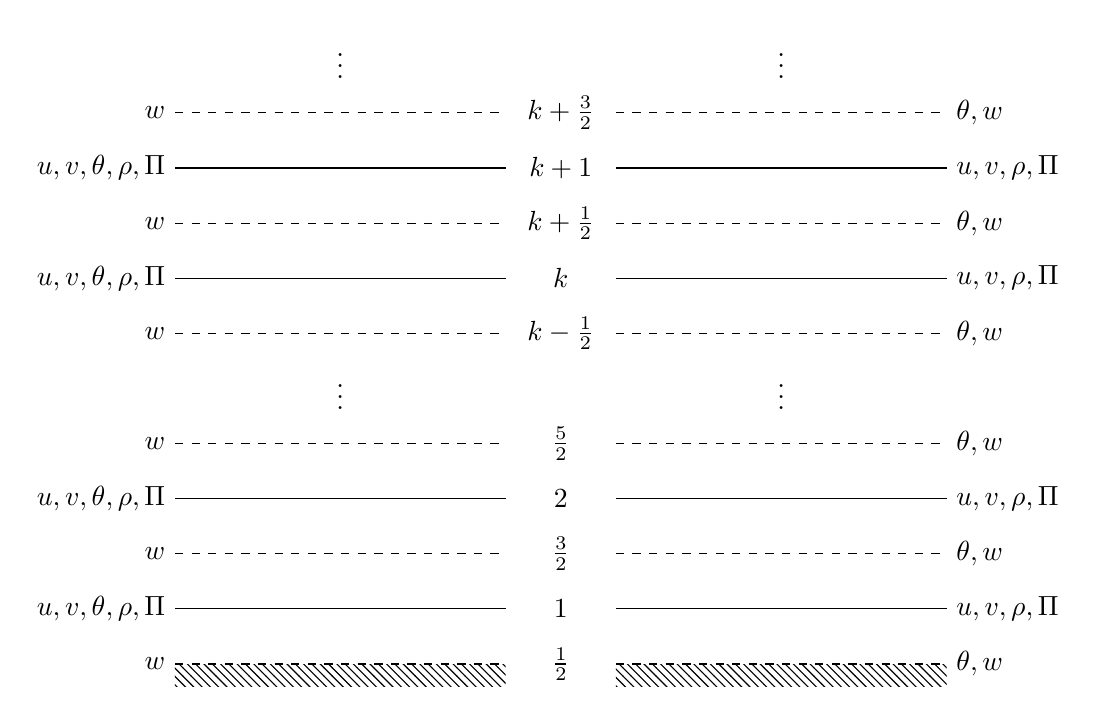
\begin{tikzpicture}[
  scale=0.7
]
\fill [pattern=north west lines] (0,0) rectangle (6,-0.4);
\fill [pattern=north west lines] (8,0) rectangle (14,-0.4);
\node at (7,0) {$\frac{1}{2}$};
\draw [dashed] (0,0) -- (6,0) node [at start, anchor=east] {$w$};
\draw [dashed] (8,0) -- (14,0) node [at end, anchor=west] {$\theta, w$};

\node at (7,1) {$1$};
\draw (0,1) -- (6,1) node [at start, anchor=east] {$u, v, \theta, \rho, \exner$};
\draw (8,1) -- (14,1) node [at end, anchor=west] {$u, v, \rho, \exner$};

\node at (7,2) {$\frac{3}{2}$};
\draw [dashed] (0,2) -- (6,2) node [at start, anchor=east] {$w$};
\draw [dashed] (8,2) -- (14,2) node [at end, anchor=west] {$\theta, w$};

\node at (7,3) {$2$};
\draw (0,3) -- (6,3) node [at start, anchor=east] {$u, v, \theta, \rho, \exner$};
\draw (8,3) -- (14,3) node [at end, anchor=west] {$u, v, \rho, \exner$};

\node at (7,4) {$\frac{5}{2}$};
\draw [dashed] (0,4) -- (6,4) node [at start, anchor=east] {$w$};
\draw [dashed] (8,4) -- (14,4) node [at end, anchor=west] {$\theta, w$};

\node at (3,5) {$\vdots$};
\node at (11,5) {$\vdots$};

\node at (7,6) {$k - \frac{1}{2}$};
\draw [dashed] (0,6) -- (6,6) node [at start, anchor=east] {$w$};
\draw [dashed] (8,6) -- (14,6) node [at end, anchor=west] {$\theta, w$};

\node at (7,7) {$k$};
\draw (0,7) -- (6,7) node [at start, anchor=east] {$u, v, \theta, \rho, \exner$};
\draw (8,7) -- (14,7) node [at end, anchor=west] {$u, v, \rho, \exner$};

\node at (7,8) {$k + \frac{1}{2}$};
\draw [dashed] (0,8) -- (6,8) node [at start, anchor=east] {$w$};
\draw [dashed] (8,8) -- (14,8) node [at end, anchor=west] {$\theta, w$};

\node at (7,9) {$k + 1$};
\draw (0,9) -- (6,9) node [at start, anchor=east] {$u, v, \theta, \rho, \exner$};
\draw (8,9) -- (14,9) node [at end, anchor=west] {$u, v, \rho, \exner$};

\node at (7,10) {$k + \frac{3}{2}$};
\draw [dashed] (0,10) -- (6,10) node [at start, anchor=east] {$w$};
\draw [dashed] (8,10) -- (14,10) node [at end, anchor=west] {$\theta, w$};

\node at (3,11) {$\vdots$};
\node at (11,11) {$\vdots$};
\end{tikzpicture}
\end{document}
